%!TEX root=./paper.tex



\subsection{Static Inference of Function Side-Effects}
\label{Se:MayMod}
\label{Se:IdentifyingLoads}
 
The auxiliary function $\Call{mayMod}{ \workstate, \funclist, \addr }$
receives as parameter a symbolic state $\workstate$, a list of skipped 
invocations $\funclist$, and an address $\addr$ which is the target of a $\instruct{Load}$ instruction,
and determines whether one of the skipped function in   $\funclist$ may store a value in $\addr$.
The function makes this decision using a \emph{points-to} graph 
computed by a preliminary stage of pointer analysis~\cite{Hind:Paste2001,Smaragdakis:FTPL2015}. 

More specifically, we perform a whole program flow-insensitive context-insensitive field-sensitive 
points-to analysis which determines, in a conservative way, the memory location each pointer variable may point-to
when the program runs.
In this analysis, memory locations are conservatively abstracted using their \emph{allocation sites}:
Every definition of a local or a global variable is considered to be an allocation site, as well as 
every program point in which memory is allocated.
For example, if the program contains a command $\code{while (\ldots) do L: p = (int*) malloc(4)}$ then 
we represent all the memory locations allocated in $L$ by a single allocation site $\mathit{AS}_L$.
We say that $\code{p}$ 
may point to allocation site $\mathit{AS}_L$, and if the 
program contains  a command of the form $\code{p=q}$, we say the same about $\code{q}$. 
The  points-to graph of a program 
contain as nodes variable names and allocation sites, and its edges represent \emph{points-to relations}:
an edge from 
a node $w$ means that the memory location represented by $v$, which can be a variable or a field of a 
(possibly dynamically allocated) \code{struct}, may hold a 
pointer to a location represented by~$w$.

The points-to graph, which  is computed once for every program,   conservatively represents all the possible points-to relation in any possible program execution.
Using the points-to graph, we use a standard \emph{may-mod} analysis (see, e.g.,~\cite{dragon-book}), in which 
we find the side effects of every function $f$, i.e.,  the set of possible locations, represented by their allocation sites,
that it, or any function that it may (transitively) invoke, may modify.




During the chopped symbolic execution, we instrument the symbolic state to record the allocation site of every 
memory location. 
\dt{This is actually done in KLEE by default \noam{We can say that in the implementation section.}}
This instrumentation, together with the program points-to graph, allows \textsc{mayMod}()
to determine whether a skipped function may, or may not, write to a given address.
Recall that the pointer analysis is flow-insensitive, and thus 
it might record that a skipped function might modify a location which is updated later on in the symbolic execution.
More specifically, a $\instruct{load}$ instruction from address $\addr$ is \emph{dependent on an invocation of a skipped function} if and only if two conditions are met: 
(1)~$\addr$ is among the 
locations that \textit{may} be modified by the skipped function (according to the may-mod analysis),
and (2)~no store to that location happened between the the skipped invocation function and the load.
In particular, when the second condition doesn't hold, no recovery is needed
as the stores done by the skipped function are irrelevant. 
$\Call{mayMod}{}$ utilizes the information gather during the dynamic symbolic execution 
regarding overwritten locations to 
refine, on the fly, the detection of the \emph{relevant} side effects of skipped functions. 
Technically, conditions (1) and (2) are checked in \cref{alg:maymod-static,alg:maymod-dynamic}
of Algorithm~\ref{fig:aux-func-may-mod},
respectively.
% stored in the overwritten addresses 

%  Otherwise, it means that the memory
% location being read by the load was written to in the skipped
% function, and the first condition should hold (the memory location
% might also be uninitialized, but this is a orthogonal problem).

%\subsection{Identifying dependent loads}\label{Se:IdentifyingLoads}

% We have not yet discussed in detail how we identify dependent loads.
% A load is dependent on a skipped function if and only if two
% conditions are met: (1)~the memory location read by the load is among
% the locations that \textit{may} be modified by the skipped function
% (\ie among $M^*_f$), and (2)~no store to that location happened between the
% call to the skipped function and the load.

% When the second condition doesn't hold, i.e. the memory location
% accessed by the load was written after the call to the skipped
% function, no recovery is needed.  Otherwise, it means that the memory
% location being read by the load was written to in the skipped
% function, and the first condition should hold (the memory location

% might also be uninitialized, but this is a orthogonal problem).


%  dynamically allocated 

% $f$ may go over all the $\instruct{Store}$ instructions in the program and determine the allocation site they may modify.


% To make this decision, we statically compute the \textit{side effects}
% of each skipped function, which are defined to be the set of memory
% locations written by that function which are accessible by the rest of
% the program.  This is achieved by a standard \textit{mod-ref
%   analysis.}

% \paragraph{Mod-ref analysis.} For simplicity, we assume that the skipped
% function $f$ under analysis has no return value, so we can only
% express the analysis in terms of load and store instructions.  The
% general case can be reduced to the no-return-value case by adding an
% out parameter.

%The analysis has the following steps:

% \begin{enumerate}[leftmargin=*]

% \item \textit{Points-to analysis. } We run a flow-insensitive
%   context-insensitive points-to analysis~\cite{dragon-book} on the
%   whole program, which will later tell us which memory locations might
%   be accessed by a given load or store.

% \item \textit{Reachability analysis.} We compute $R_f$, the set of
%   functions that $f$ might call (including $f$ itself).  This is
%   needed because the side effects of $f$ depend on the side effects of
%   $R_f$.

% \item \textit{Ref-set of whole program.}  We next compute the
%   \textit{ref-set} of the whole program ($Ref$), \ie the set of
%   locations that are read throughout the program.  This is simply the
%   union of all the points-to sets of all the load instructions in the
%   program.

% \item \textit{Mod-set of $f$.}  We compute the \textit{mod-set} of
%   $f$, denoted by $M_f$, which is the set of locations that $f$ may
%   modify.  $M_f$ is the union of all the points-to sets of all the
%   store instructions in $f$.  The \textit{inclusive modifies set} for
%   $f$ is $M^{*}_f = \cup_{g \in R_f} M_g$.

% \item \textit{Side effects of $f$.}  The side effects of $f$, \ie the
%   set of memory locations written by $f$ which are accessible by the
%   rest of the program, is then simply $SE_f = M^{*}_f \cap Ref$.

% \end{enumerate}

\subsection{Multiple recovery states.} 
In some cases, we need to create
several recovery states. 
For example, function $\code{g()}$ in Figure~\ref{fig:multiple-recoveries} 
invokes function $\code{f}()$, shown in Figure~\ref{fig:simple}, twice.
If we wish to skip invocations of $\code{f}()$ then
two recovery states are created:
one at \text{line 6} and another at \text{line 9}.  Suppose that
the first recovery state modifies the value of $\code{p.x}$ executes \text{line 3} in the slice of $f$.
If the second recovery state chooses the path which goes through
\textit{line 5}, then we get an infeasible path.  In order to avoid
such situations, a recovery state adds its new constraints to the
\textit{guiding constraints} of its dependent state.  The guiding
constraints will be used in subsequent recovery states.  In our
example, the constraint $k > 0$ will be added to the guiding
constraints, so the second recovery state will be forced to go through
\textit{line 3}.


\begin{figure}[tbp]
  \lstinputlisting[linewidth=.95\columnwidth]{code/multiple-recov.c}
\caption{Multiple recovery states for a single function.}
\label{fig:multiple-recoveries}
\end{figure}

\begin{figure}[tbp]
  \lstinputlisting[linewidth=.95\columnwidth]{code/allocations.c}
\caption{Executing slices with allocations.}
\label{fig:slices-with-allocations}
\end{figure}



\noam{I am here.}


\subsection{TODO}

With the side effects of each skipped functions computed, we can start
the recovery from the first skipped function (first in the order in
which the functions were skipped) whose side effects include the
memory location accessed by the dependent load.  Note that, we cannot
start from the last such function, because we cannot determine
statically whether that function would actually modify that memory
location.



\begin{figure}[tbp]
\lstinputlisting[linewidth=.95\columnwidth]{code/multiple-skipped.c}
\caption{Multiple skipped functions.}
\label{fig:multiple-skipped-functions}
\end{figure}


Another aspect that we need to handle are dependencies between
skipped functions.  When we create a recovery state for a skipped
function which is not the first skipped function, the recovery state
might be dependent on previously skipped functions.  In this case, we
have to apply our technique recursively and treat the recovery state
as a \textit{dependent} state.  For instance, consider the code in
Figure~\ref{fig:multiple-skipped-functions}.  When we reach the
dependent load at \textit{line 16}, we create a recovery state for
$f_2$, since $f_1$ does not modify the field $x$.  When the created
recovery state reaches the load instruction at \textit{line 6}, it
identifies it as a dependent load.  It then creates another recovery
state which executes $f_1$.  Once the recovery of $f_1$ is completed
we can continue the execution of the recovery in $f_2$.

\paragraph{Optimizations.} For a given state, we create a cache which
remembers which recovery states were actually relevant for a given
load.  By doing this, we can avoid redundant recovery executions.
This basic caching can be improved, by caching the expression which
was written (if it was written) during the execution of a slice.




\ignore{
\subsection{Handling Multiple Skipped Functions}
\label{Se:MayMod}
\label{Se:IdentifyingLoads}
\label{Se:SkipMultipleFuncs}

So far, we have assumed a single skipped function $f$.  If instead we
skip multiple functions $f_1, f_2, \ldots$, we need to decide which
functions need to be recovered, and in particular from the snapshot of
whose function to create the recovery state.  Note that while it would
be correct to start from the first skipped function, this would be
highly inefficient.

To make this decision, we statically compute the \textit{side effects}
of each skipped function, which are defined to be the set of memory
locations written by that function which are accessible by the rest of
the program.  This is achieved by a standard \textit{mod-ref
  analysis.}

\paragraph{Mod-ref analysis.} For simplicity, we assume that the skipped
function $f$ under analysis has no return value, so we can only
express the analysis in terms of load and store instructions.  The
general case can be reduced to the no-return-value case by adding an
out parameter.

The analysis has the following steps:

\begin{enumerate}[leftmargin=*]

\item \textit{Points-to analysis. } We run a flow-insensitive
  context-insensitive points-to analysis~\cite{dragon-book} on the
  whole program, which will later tell us which memory locations might
  be accessed by a given load or store.

\item \textit{Reachability analysis.} We compute $R_f$, the set of
  functions that $f$ might call (including $f$ itself).  This is
  needed because the side effects of $f$ depend on the side effects of
  $R_f$.

\item \textit{Ref-set of whole program.}  We next compute the
  \textit{ref-set} of the whole program ($Ref$), \ie the set of
  locations that are read throughout the program.  This is simply the
  union of all the points-to sets of all the load instructions in the
  program.

\item \textit{Mod-set of $f$.}  We compute the \textit{mod-set} of
  $f$, denoted by $M_f$, which is the set of locations that $f$ may
  modify.  $M_f$ is the union of all the points-to sets of all the
  store instructions in $f$.  The \textit{inclusive modifies set} for
  $f$ is $M^{*}_f = \cup_{g \in R_f} M_g$.

\item \textit{Side effects of $f$.}  The side effects of $f$, \ie the
  set of memory locations written by $f$ which are accessible by the
  rest of the program, is then simply $SE_f = M^{*}_f \cap Ref$.

\end{enumerate}

With the side effects of each skipped functions computed, we can start
the recovery from the first skipped function (first in the order in
which the functions were skipped) whose side effects include the
memory location accessed by the dependent load.  Note that, we cannot
start from the last such function, because we cannot determine
statically whether that function would actually modify that memory
location.
}



\subsection{Memory allocations} \label{Se:Malloc}

Let us consider the example
from Figure~\ref{fig:slices-with-allocations}.  After skipping the
function call for $f$, the first dependent load instruction is at
\textit{line 14}, and the second one at \textit{line 15}.
If \textit{malloc} returned a different address while executing the
second recovery state, this may lead to undefined behavior.
To prevent this and maintain consistency across recovery states
originating from the same function call, for each allocation site in
$f$, we maintain a list of returned addresses.  An allocation site is
identified by its call stack.  This way, the subsequent recovery
states will use this information while re-executing allocating
instructions.

 



\subsection{Skipping Multiple Functions}\label{Se:SkipMultipleFuncs}

So far, we have assumed a single skipped function $f$.  If instead we
skip multiple functions $f_1, f_2, \ldots$, we need to decide which
functions need to be recovered, and in particular from the snapshot of
whose function to create the recovery state.  Note that while it would
be correct to start from the first skipped function, this would be
highly inefficient.

To make this decision, we statically compute the \textit{side effects}
of each skipped function, which are defined to be the set of memory
locations written by that function which are accessible by the rest of
the program.  This is achieved by a standard \textit{mod-ref
  analysis.}

\paragraph{Mod-ref analysis.} For simplicity, we assume that the skipped
function $f$ under analysis has no return value, so we can only
express the analysis in terms of load and store instructions.  The
general case can be reduced to the no-return-value case by adding an
out parameter.

The analysis has the following steps:

\begin{enumerate}[leftmargin=*]

\item \textit{Points-to analysis. } We run a flow-insensitive
  context-insensitive points-to analysis~\cite{dragon-book} on the
  whole program, which will later tell us which memory locations might
  be accessed by a given load or store.

\item \textit{Reachability analysis.} We compute $R_f$, the set of
  functions that $f$ might call (including $f$ itself).  This is
  needed because the side effects of $f$ depend on the side effects of
  $R_f$.

\item \textit{Ref-set of whole program.}  We next compute the
  \textit{ref-set} of the whole program ($Ref$), \ie the set of
  locations that are read throughout the program.  This is simply the
  union of all the points-to sets of all the load instructions in the
  program.

\item \textit{Mod-set of $f$.}  We compute the \textit{mod-set} of
  $f$, denoted by $M_f$, which is the set of locations that $f$ may
  modify.  $M_f$ is the union of all the points-to sets of all the
  store instructions in $f$.  The \textit{inclusive modifies set} for
  $f$ is $M^{*}_f = \cup_{g \in R_f} M_g$.

\item \textit{Side effects of $f$.}  The side effects of $f$, \ie the
  set of memory locations written by $f$ which are accessible by the
  rest of the program, is then simply $SE_f = M^{*}_f \cap Ref$.

\end{enumerate}

With the side effects of each skipped functions computed, we can start
the recovery from the first skipped function (first in the order in
which the functions were skipped) whose side effects include the
memory location accessed by the dependent load.  Note that, we cannot
start from the last such function, because we cannot determine
statically whether that function would actually modify that memory
location.



\begin{figure}[tbp]
\lstinputlisting[linewidth=.95\columnwidth]{code/multiple-skipped.c}
\caption{Multiple skipped functions.}
\label{fig:multiple-skipped-functions}
\end{figure}


Another aspect that we need to handle are dependencies between
skipped functions.  When we create a recovery state for a skipped
function which is not the first skipped function, the recovery state
might be dependent on previously skipped functions.  In this case, we
have to apply our technique recursively and treat the recovery state
as a \textit{dependent} state.  For instance, consider the code in
Figure~\ref{fig:multiple-skipped-functions}.  When we reach the
dependent load at \textit{line 16}, we create a recovery state for
$f_2$, since $f_1$ does not modify the field $x$.  When the created
recovery state reaches the load instruction at \textit{line 6}, it
identifies it as a dependent load.  It then creates another recovery
state which executes $f_1$.  Once the recovery of $f_1$ is completed
we can continue the execution of the recovery in $f_2$.

\paragraph{Optimizations.} For a given state, we create a cache which
remembers which recovery states were actually relevant for a given
load.  By doing this, we can avoid redundant recovery executions.
This basic caching can be improved, by caching the expression which
was written (if it was written) during the execution of a slice.



% \subsection{Identifying dependent loads}\label{Se:IdentifyingLoads}

% We have not yet discussed in detail how we identify dependent loads.
% A load is dependent on a skipped function if and only if two
% conditions are met: (1)~the memory location read by the load is among
% the locations that \textit{may} be modified by the skipped function
% (\ie among $M^*_f$), and (2)~no store to that location happened between the
% call to the skipped function and the load.

% When the second condition doesn't hold, i.e. the memory location
% accessed by the load was written after the call to the skipped
% function, no recovery is needed.  Otherwise, it means that the memory
% location being read by the load was written to in the skipped
% function, and the first condition should hold (the memory location
% might also be uninitialized, but this is a orthogonal problem).




\subsection{Slice selection}\label{Se:Slicing}

Recall from the overview that ...

More formally, let $MR_{f,l}$ be the intersection of the points-to set
of $l$ with $M^{*}_f$.  Then, we construct the set of all store
instructions in $R_f$ whose points-to sets intersect with $MR_{f,l}$.
This set of store instructions is then the input to a standard
static slicing algorithm which will slice the functions in $R_f$ with
respect to this set (\ie the algorithm will remove any statements from
$R_f$ which are unrelated to these store instructions).

%!TEX root=./paper.tex

\subsection{Chopping-Aware Search Heuristics}
\label{Se:Search}

Search heuristics are the main approach to reduce path explosion and
steer symbolic execution to uncovered paths for a more effective
exploration~\cite{exe,klee,sen:concolicheuristics,fitsymex:dsn09}, and
chopped symbolic execution is no exception. However, these heuristics
do not take into account the particular nature of the states in
chopped symbolic execution, that is the distinction between normal and
recovery states.

We propose a \textit{chopping-aware} search heuristic, which attempts
to optimize the exploration of chopped symbolic execution, while
aiming to a faster recovery of side effects. The heuristic's behavior
crucially depends on the current state being executed. Under normal
conditions---that is while symbolically executing normal states---the
search heuristic favors the selection of normal states at the next
steps. The rationale is that we want to favor paths that do not
require any recovery, thus fostering code exploration.

Instead, when chopped symbolic execution is executing a recovery
state, the search heuristic only selects the recovery states involved
in the recovery process. In this case, we want to favor a fast
recovery of the side effects needed by the dependent state. As soon as
the recovery state terminates, the search heuristic will switch to the
normal behavior.

Since always favoring normal states over recovery states may lead to
saturation in code exploration, we allow the searcher to select at a
lower probability a recovery state even under normal execution
conditions.

%%% Local Variables:
%%% mode: latex
%%% TeX-master: "paper"
%%% End:




%% \paragraph{Detecting overriding stores.} We might have a load instruction
%% which is dependent according to the static analysis, but recovery is
%% not required.  For example if there the value was written between the
%% skipped function and the dependent load.  In fact, executing a
%% recovery state in this case may lead to incorrect results.  We collect
%% for each load instruction, the store instructions which may collide
%% with it.  When a state executes a may-colliding store instruction, it
%% remembers the address and the size.  This way, when a load instruction
%% is encountered, we are able to determine if the read value was
%% overridden or not.  Note that not all store instructions should be
%% considered, but only those which may collide with a relevant load
%% instruction.  The overriding stores are computed as part of the
%% mod-ref analysis.



% Let $main$ be the entry point of the program and $f$ be a function
% which we would like to skip.  We start executing $main$ symbolically.
% When a state reaches the function call for $f$, we create a
% \textit{snapshot state} using the current state and skip the function
% call.  We continue the execution of the state, but from this point we
% must remember that some load instructions may depend on the
% \textit{side effects} of the skipped function $f$.

% %% When we have a fork in a recovery state, we fork the recovery state as
% %% in the usual case.  In the original recovery state, we add the
% %% corresponding condition to its dependent state as well.  In the case
% %% of the newly created recovery state, we fork the dependent state of
% %% the original recovery state and set it to be the dependent state of
% %% the new recovery state.  The corresponding condition is added to the
% %% forked dependent state as well as to the new recovery state.


% \begin{figure*}[t]
%   \centering
%   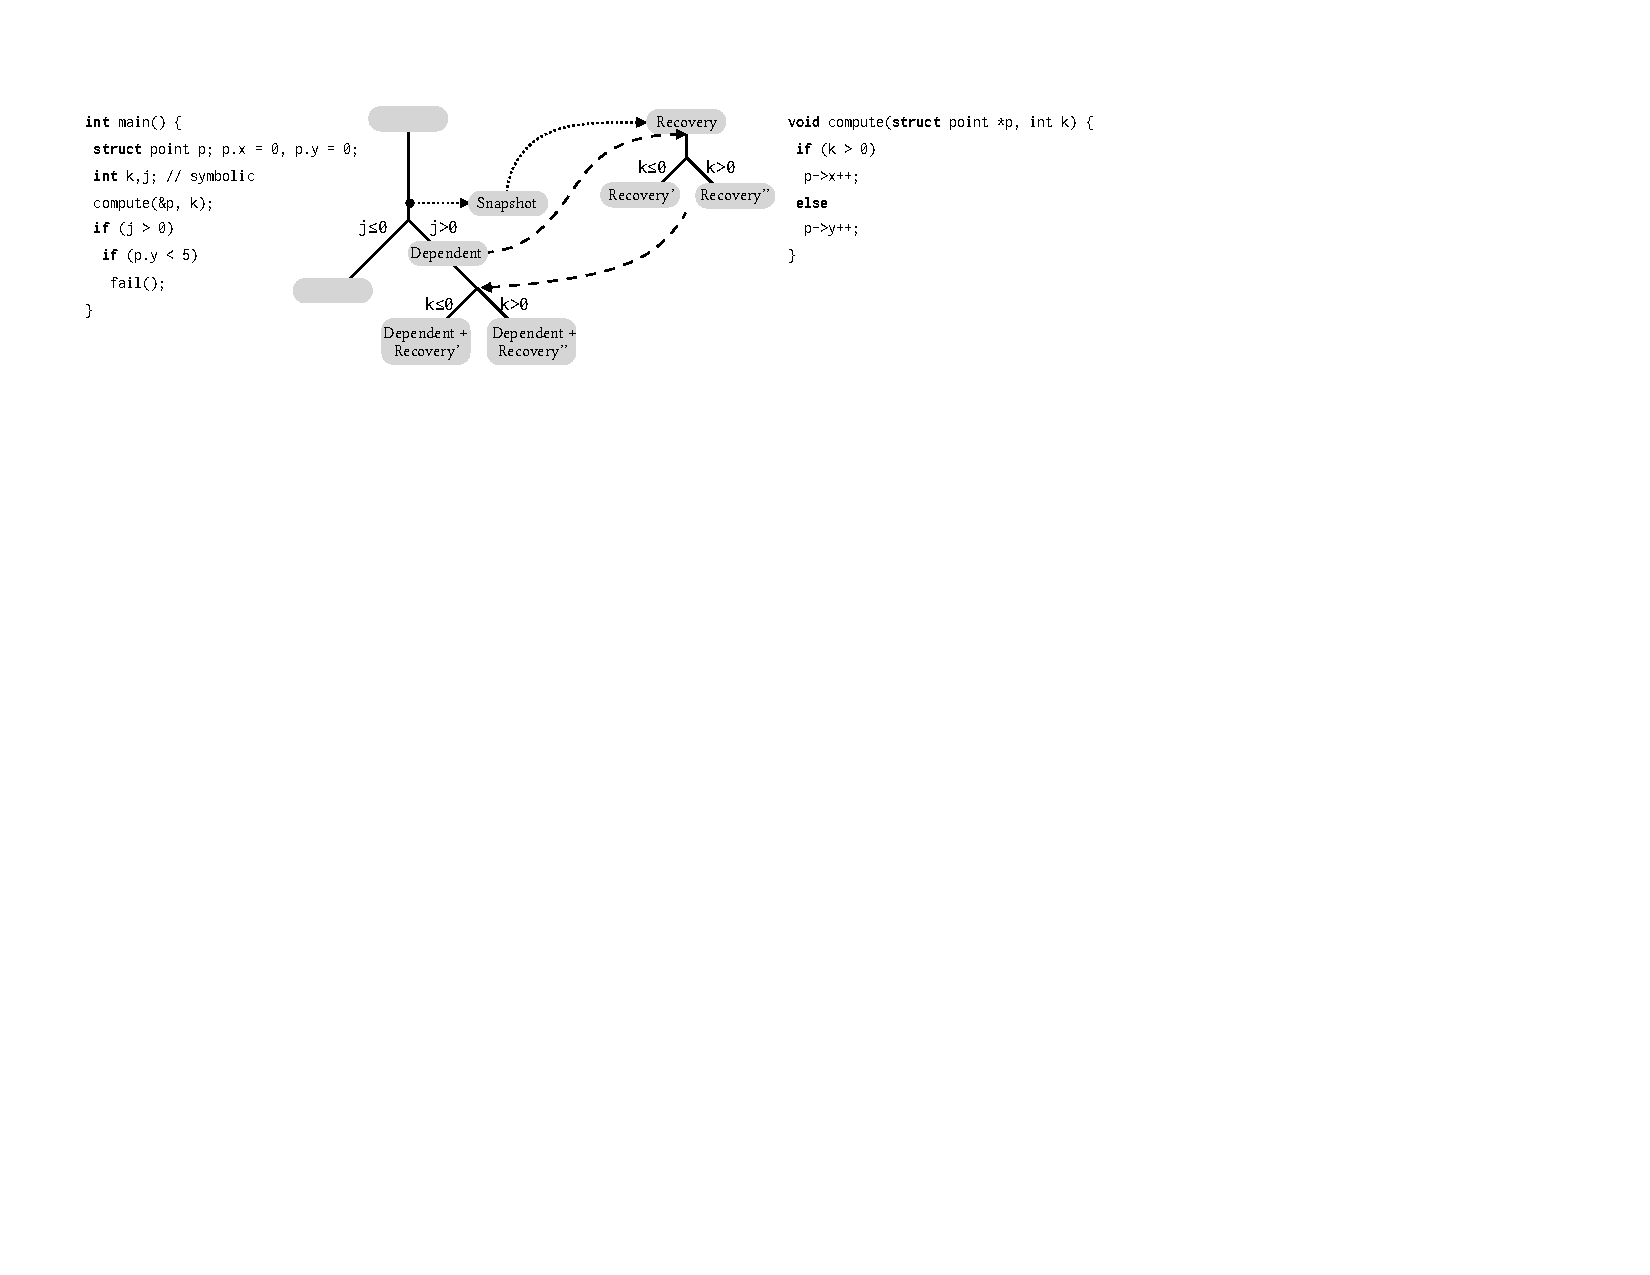
\includegraphics[width=.95\textwidth]{img-states2}
%   \caption{Graphical illustration of snapshot, dependent and recovery states.}
%   \label{fig:cse-states}
% \end{figure*}

% When such a \textit{dependent load} is encountered, the state, which
% now becomes a \textit{dependent state} is suspended. At this point, we
% create a new \textit{recovery state} which inherits the snapshot state
% of $f$ and execute symbolically function $f$.
% Figure~\ref{fig:cse-states} shows the relationship between the
% \textit{snapshot state}, \textit{dependent state} and \textit{recovery
%   state} in a graphical way.

% %% For example, if the load instruction which caused the creation
% %% of the recovery state reads $n$ bytes from the address $a$, then the
% %% recovery state updates the dependent state only on store instructions
% %% which write to the range $[a, a + n]$.

% While symbolically running the recovery state, if execution forks,
% then the same fork is performed in the dependent state.  Furthermore,
% as we run the recovery state, any stores to the memory location read
% by the dependent load are also performed in the dependent state.
% %
% If the recovery state returns successfully, the dependent state is
% resumed successfully.  If an error occurs while executing the recovery
% state (\eg an invalid memory access) the dependent state is
% terminated.

% When we execute a recovery state, not all paths will be compatible
% with the execution which the dependent state reached.  For instance,
% the dependent state might contain the constraint that $x>0$ which was
% added after the function $f$ was skipped. One option would be to
% execute during recovery all possible paths thorough $f$, and later
% filter the ones that are incompatible with the dependent state.
% However, this would potentially explore a large number of infeasible
% paths, so we designed a more efficient solution.  Each state maintains
% a list of \textit{guiding constraints} which were added since the call
% to the skipped function.  Before we start executing a recovery state,
% we add these \textit{guiding constraints} from the dependent state to
% the path constraints of the recovery state.  By doing this, we
% guarantee that every path explored in the recovery state is consistent
% with respect to its dependent state.
 
% \begin{figure}[tbp]
%   \lstinputlisting[linewidth=.95\columnwidth]{code/multiple-recov.c}
% \caption{Multiple recovery states for a single function.}
% \label{fig:multiple-recoveries}
% \end{figure}

% \paragraph{Multiple recovery states.}  
% In some cases we need to create
% several recovery states. For example, in
% Figure~\ref{fig:multiple-recoveries} two recovery states are created,
% one at \textit{line 14} and another at \textit{line 17}.  Suppose that
% the first recovery state executes \textit{line 3} in the slice of $f$.
% If the second recovery state chooses the path which goes through
% \textit{line 5}, then we get an infeasible path.  In order to avoid
% such situations, a recovery state adds its new constraints to the
% \textit{guiding constraints} of its dependent state.  The guiding
% constraints will be used in subsequent recovery states.  In our
% example, the constraint $k > 0$ will be added to the guiding
% constraints, so the second recovery state will be forced to go through
% \textit{line 3}.


% \begin{figure}[tbp]
%   \lstinputlisting[linewidth=.95\columnwidth]{code/allocations.c}
% \caption{Executing slices with allocations.}
% \label{fig:slices-with-allocations}
% \end{figure}



% \paragraph{Memory allocations.} Let us consider the example
% from Figure~\ref{fig:slices-with-allocations}.  After skipping the
% function call for $f$, the first dependent load instruction is at
% \textit{line 14}, and the second one at \textit{line 15}.
% %% The corresponding slice contains only \textit{line~4}.
% %% The second dependent load instruction is at
% %% and its slice contains only \textit{lines 4,5}.  Note that in this
% %% case, the allocation appears in both slices.
% If \textit{malloc} returned a different address while executing the
% second recovery state, this may lead to undefined behaviour.
% %% Our observation is that if two slices have a common allocation site, then
% %% in both slices it is executed the same number of times.
% To prevent this and maintain consistency across recovery states
% originating from the same function call, for each allocation site in
% $f$, we maintain a list of returned addresses.  An allocation site is
% identified by its call stack.  This way, the subsequent recovery
% states will use this information while re-executing allocating
% instructions.
% }


%%We map the load instruction $l$ to the allocation sites of the
%% pointers in $MR_{f,l}$.  This mapping will help us to determine at
%% runtime if the skipped function $f$ requires recovery.  Each such
%% allocation site is mapped to the store instructions in the skipped
%% function (including any reachable functions) which may modify it.
%% This mappings will be used to define the slicing criterion for $f$.

% \begin{algorithm}[tbp]
% \caption{pseudo code}
% \begin{algorithmic}[1]
% \Function{exeucteNormalState}{}
% \If{current instruction is a call}
%   \If{called function should be skipped}
%     \State create a snapshot of the current state
%   \Else
%     \State execute call instruction
%   \EndIf
% \EndIf
% \If{current instruction is a load}
%   \If{no function was skipped}
%     \State execute load instruction
%   \Else
%     \State $as \gets$ the exact allocation site of the load operand
%     \State $slice \gets$ the slice which corresponds to $as$
%     \State suspend current state
%     \State \Call{startRecoveryState}{$slice$}
%   \EndIf
% \EndIf
% \If{current instruction is a store}
%   \If{at least one function was skipped}
%     \If{the store may-override}
%       \State add the overriden address to the current state
%     \EndIf
%   \EndIf
%   \State execute store instruction
% \EndIf
% \EndFunction
% \label{fig:pseudo-code-1}
% \end{algorithmic}
% \end{algorithm}

% \begin{algorithm}[tbp]
% \caption{pseudo code}
% \begin{algorithmic}[1]
% \Function{exeucteRecoveryState}{$s$}
% \If{current instruction is a store}
%   \State{execute store instruction}
%   \State $addr \gets$ the address of the store operand
%   \If{$addr$ is the blocking address}
%     \State update the written value in the dependent state of $s$
%   \EndIf
% \EndIf
% \If{current instruction is the exit point of the slice}
%   \State terminate $s$
%   \State resume the dependent state of $s$
% \EndIf
% \If{current instruction is a branch}
%   \State $s' \gets$ \Call{fork}{$s$}
%   \State $ds \gets$ the dependent state of $s$
%   \State $ds' \gets$ \Call{fork}{$ds$}
%   \State add the condition to $s$ and $ds$
%   \State add the negated condition to $s'$ and $ds'$
% \EndIf
% \EndFunction
% \end{algorithmic}
% \label{fig:pseudo-code-2}
% \end{algorithm}

% \begin{algorithm}[tbp]
% \caption{pseudo code}
% \begin{algorithmic}[1]
% \Function{startRecoveryState}{$ds$, $slice$}
% \State $snapshot \gets$ the snapshot from the skipped call site
% \State $rs \gets$ \Call{fork}{$snapshot$}
% \State $gc \gets$ the guiding constraints of the dependent state of $rs$
% \State add $gc$ to the path constraints of $rs$
% \State add $rs$ to the pool of states
% \EndFunction
% \end{algorithmic}
% \label{fig:pseudo-code-3}
% \end{algorithm}

%%% Local Variables:
%%% mode: latex
%%% TeX-master: "paper"
%%% End:
